\documentclass[11pt]{article}

\usepackage[a4paper,margin=2.5cm]{geometry}
\usepackage[T1]{fontenc}
\usepackage{lmodern}
\usepackage{microtype}
\usepackage{amsmath,amssymb,amsthm}
\usepackage{booktabs}
\usepackage{xspace}
\usepackage{pgfplots}
\usepackage[hidelinks]{hyperref}
\pgfplotsset{compat=1.18}
\usetikzlibrary{arrows.meta}

\def\..{\,\mathpunct{\ldotp\ldotp}} % Middle stuff for intervals. Usage: \..

\newcommand{\PHast}{PHast\xspace}
\newcommand{\PHastP}{PHast$^+$\xspace}
\newcommand{\PHastR}{PHast-R\xspace}
\newcommand{\hi}{\operatorname{hi}}
% Shifts as binary operators
\DeclareMathSymbol{\ll}{\mathbin}{symbols}{"1C}
\DeclareMathSymbol{\gg}{\mathbin}{symbols}{"1D}
\newtheorem{proposition}{Proposition}

\title{\PHastR: Bit--Parallel Perfect Hashing\\with Rings of Patterns}
\author{Sebastiano Vigna\\Dipartimento di Informatica, Università degli Studi di Milano}
\date{}

\begin{document}
\bibliographystyle{plain}
\maketitle

\begin{abstract}
We present \PHastR, a minimal perfect hash function of the \PHast family. Like
\PHastP, the fast-to-build variant of \PHast, \PHastR finds feasible seeds with
bit-parallel operations: its seeds move keys along \emph{rings} of slots, and
to evaluate the seeds of a bucket it rotates, for each key, a word recording
which slots of its ring are used. Unlike \PHastP, however, it avoids
\emph{self-collisions}, which make two keys of a bucket collide for (almost)
all its seeds, and cause almost $40\%$ of the bumping of \PHastP with
wrapping. With 8-bit seeds, \PHastR uses $1.93$ bits per key against the
$1.97$ of \PHastP with wrapping, it is built in half the time, and its queries
are faster; its space and its query time are close to those of \PHast, which
takes more than ten times as long to build. With 10-bit seeds it uses $1.85$
bits per key against $1.87$. Finally, we prove that when each key can be
placed only within a window of $W$ slots, every placement of $n$ random keys
on $n$ slots, however found, bumps on average at least about $\sqrt{\pi n/2}-W$ keys.
\end{abstract}

\section{Introduction}

A \emph{minimal perfect hash function} (MPHF) maps a static set of $n$ keys
bijectively to $[0\..n)$; it requires at least $\lg e\approx 1.443$
bits per key (we use $\lg$ for the binary logarithm and $\ln$ for the natural
logarithm). Among the many practical constructions, \emph{bucket placement}
gives the fastest queries: keys are hashed to buckets, and a per-bucket seed
chooses positions for the keys of the bucket so that no two keys collide.
The idea goes back to FCH~\cite{FCHFACMPHF}, whose construction, however,
was slow and needed a lot of space; the idea received little attention until
PTHash~\cite{PTPRFMPH} brought it back, followed by many others, such as PHOBIC~\cite{HLPPPHOBSIC}
and PtrHash~\cite{RagPTR}.

\PHast~\cite{BeSPHast} pushes this approach to its limit: the seeds are
stored in a plain array of fixed-width values, each seed places the keys of
its bucket inside small overlapping slices of the output range, and a query
reads a single seed for almost all keys. Finding the seeds, however, is
expensive, as \PHast tries all the seeds of each bucket: construction takes
hundreds of nanoseconds per key. Its variant \PHastP finds feasible seeds
with bit-parallel operations, and it is an order of magnitude faster to
build, but with 8-bit seeds it needs $2.12$ bits per key instead of $1.92$,
or $1.97$ in its variants with wrapping, which are slower to build.

In this paper we present \PHastR, a structure of the same family with the
space and the query time of \PHast and a construction faster than that of
\PHastP. This paper makes four contributions:
\begin{itemize}
\item \PHastR, a structure in which the lowest bits of the seed of a bucket
choose one of $R$ independent patterns, and the remaining bits a rotation,
which moves each key of the bucket along a ring of slots; rings make it
possible to find all the rotations of a pattern that map no key to a used
slot by rotating blocks of bits (Section~\ref{sec:phastr});
\item an analysis of the differences from \PHast and \PHastP, showing that
the excess space of \PHastP, with and without wrapping, comes from bumping,
that a large part of the bumping is caused by self-collisions inherent to
additive placement, and that patterns make their effect negligible
(Section~\ref{sec:differences});
\item an implementation in the Rust crate \texttt{sux}, an experimental
comparison with the reference implementation of \PHast and \PHastP
(Section~\ref{sec:experiments}), and an offline construction that reads the
keys just once, needs less than a byte per key of memory, and builds the same
structure as the construction in memory (Section~\ref{sec:offline});
\item a lower bound on the number of bumped keys that holds for every placement
in which each key can be placed only within a window of fixed length, which
implies that on large
key sets no search can produce a first level free of bumping
(Section~\ref{sec:limits}).
\end{itemize}

\section{\PHastR}
\label{sec:phastr}

\PHastR follows the scheme of \PHast~\cite{BeSPHast}; we discuss the
differences in Section~\ref{sec:differences}. Each key has a $64$-bit hash,
which determines its \emph{bucket}, among $B$ buckets, and its \emph{slice},
a range of $L$ consecutive slots of the output range $[0\..m)$ whose start
grows linearly with the hash. Each bucket has a seed, stored in a plain array
of $S$-bit values, which places the keys of the bucket in their slices; a
seed is \emph{feasible} for a bucket if it maps its keys to distinct free
slots. Buckets for which no seed is feasible are \emph{bumped} (seed~$0$),
and their keys are handled by further levels. The first level has output
range $m=n$, so every bumped key leaves a free slot (a \emph{hole}) in the
first level, and an Elias--Fano sequence~\cite{EliESRCASF,FanNBRISM} maps the
outputs of the further levels to the holes. Since bumped keys are few, a query
reads a single seed for almost all keys. Seeds are assigned by a sweep over
the buckets, which keeps a small window of buckets in a priority queue that
favors large buckets, and chooses for each bucket the feasible seed
minimizing the sum of the slots of its keys.

Each hole costs about $2+\lg(1/\beta)$ bits in the Elias--Fano remapping,
where $\beta$ is the fraction of bumped keys, and the bumped keys must be
placed again by the following levels, which in turn bump a fraction $\beta$
of their keys, so that overall the levels place about
$n(1+\beta+\beta^2+\cdots)=n/(1-\beta)$ keys. With $S$-bit seeds and expected
bucket size $\lambda=n/B$ the seeds take $S/\lambda$ bits for each key placed,
and the space in bits per key is thus approximately
\begin{equation}
\label{eq:space}
\frac{S}{\lambda(1-\beta)} + \beta\Bigl(2+\lg\frac1\beta\Bigr),
\end{equation}
and since the entropy of a random set of $\beta n$ holes is already about
$\beta n(\lg(1/\beta)+\lg e)$, the encoding of holes cannot be
substantially improved: once $S$ and $\lambda$ are fixed, \emph{the only
lever is $\beta$}. We will show in Section~\ref{sec:limits} that on large key
sets no placement, however found, can avoid bumping altogether; the purpose of
the design of \PHastR is to bump few keys while finding feasible seeds with
bit-parallel operations.

\begin{figure}[t]
\centering
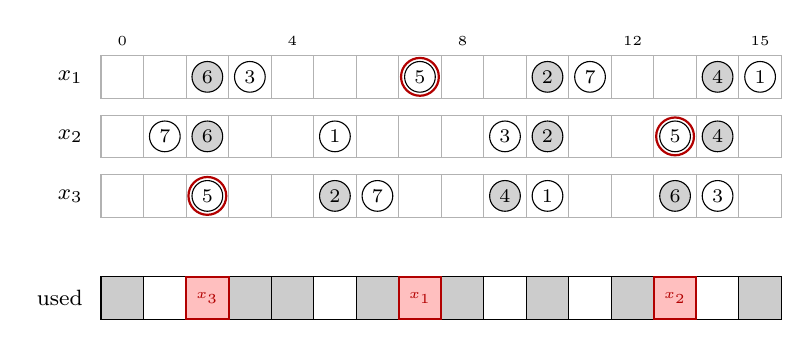
\begin{tikzpicture}[x=5.4mm,y=5.4mm,font=\footnotesize,
  p0/.style={circle,draw,fill=gray!35,inner sep=0pt,minimum size=3.9mm,font=\scriptsize},
  p1/.style={circle,draw,fill=white,inner sep=0pt,minimum size=3.9mm,font=\scriptsize}]
% Three keys with the same slice (L = 16), S = 3, R = 2: the offset for seed s
% is (omega_r + 2s) mod 16, where r = s mod 2. Offsets: x1 (6, 13), x2 (6, 3),
% x3 (1, 8).
\foreach \y/\k in {5.2/1,3.8/2,2.4/3} {
  \node[left] at (-.2,\y+.5) {$x_\k$};
  \foreach \i in {0,...,15} \draw[gray!60] (\i,\y) rectangle ++(1,1);
}
\foreach \i in {0,4,8,12,15} \node[above,font=\tiny] at (\i+.5,6.2) {$\i$};
% x1: pattern 0 (seeds 2, 4, 6) at 10, 14, 2; pattern 1 (1, 3, 5, 7) at 15, 3, 7, 11
\foreach \p/\s in {10/2,14/4,2/6} \node[p0] at (\p+.5,5.7) {$\s$};
\foreach \p/\s in {15/1,3/3,7/5,11/7} \node[p1] at (\p+.5,5.7) {$\s$};
% x2: pattern 0 at 10, 14, 2; pattern 1 at 5, 9, 13, 1
\foreach \p/\s in {10/2,14/4,2/6} \node[p0] at (\p+.5,4.3) {$\s$};
\foreach \p/\s in {5/1,9/3,13/5,1/7} \node[p1] at (\p+.5,4.3) {$\s$};
% x3: pattern 0 at 5, 9, 13; pattern 1 at 10, 14, 2, 6
\foreach \p/\s in {5/2,9/4,13/6} \node[p0] at (\p+.5,2.9) {$\s$};
\foreach \p/\s in {10/1,14/3,2/5,6/7} \node[p1] at (\p+.5,2.9) {$\s$};
% Used slots, and the slots chosen by seed 5
\node[left] at (-.2,.5) {used};
\foreach \i in {0,3,4,6,8,10,12,15} \fill[gray!40] (\i,0) rectangle ++(1,1);
\foreach \i in {0,...,15} \draw (\i,0) rectangle ++(1,1);
\foreach \p/\k in {7/1,13/2,2/3}
  \draw[red!70!black,thick,fill=red!25] (\p,0) rectangle ++(1,1)
    node[midway,font=\tiny,text=red!70!black] {$x_\k$};
\foreach \p/\y in {7/5.7,13/4.3,2/2.9}
  \draw[red!70!black,thick] (\p+.5,\y) circle (2.4mm);
\end{tikzpicture}
\caption{\label{fig:placement}The slots of the three keys $x_1$, $x_2$, $x_3$
of a bucket for each seed, with $3$-bit seeds, $R=2$ patterns, and slices of
length $L=16$ (for simplicity, the three slices coincide). Even seeds (gray)
choose pattern $0$, odd seeds (white) pattern $1$: seed $s=2j+r$ chooses
pattern $r$ and rotation $j$, which moves the keys by $jT$ slots from their
base positions, where $T=4$ is the stride, so in each pattern a key goes
through the four slots of its ring (only three of them in pattern $0$, as
seed $0$ is not available). In pattern $0$ the keys $x_1$ and $x_2$ have the same base
position, so they collide for all even seeds; in pattern~$1$ they do not. The
last row shows the slots that are already used: the only feasible seed is
$5$.}
\end{figure}

\paragraph{Placement.}
We denote with $\hi(x)$ and $\operatorname{lo}(x)$ the upper and lower $64$
bits of a $128$-bit product. Let $h$ be the hash of a key, and let
$\alpha=h/2^{64}\in[0\..1)$. The bucket of the key is $\lfloor\alpha
B\rfloor$, which in fixed-point arithmetic is just $\hi(hB)$, and the start of
its slice is $\sigma(h)=\lfloor\alpha(m-L+1)\rfloor$, which is
$\hi(h(m-L+1))$; the slice length is $L=2^\ell$. Moreover, the key has
$R=2^\rho$ independent in-slice offsets, which define $R$ \emph{patterns} of
offsets for the keys of a bucket: letting $o=\operatorname{lo}(hB)$, the
offset of the key in pattern $r\in[0\..R)$ is
\[
\omega_r(o)=(o\gg 64r/R) \bmod L,
\]
that is, the $\ell$ bits of $o$ starting at bit $64r/R$. We require
$R\ell\le 64$, so that the offsets of different patterns are disjoint blocks
of bits of $o$.

The seed $s\in[1\..2^S)$ of a bucket has two parts: its lowest $\rho$ bits,
$r=s\bmod R$, choose a pattern, and its remaining bits,
$j=s\gg\rho\in[0\..2^{S-\rho})$, a \emph{rotation}. Assuming for the
time being that $\ell\geq S$, the seed maps each key of the bucket to the slot
\[
\sigma(h)+\bigl(\omega_r(o)+(s\ll(\ell-S))\bigr)\bmod L
=\sigma(h)+\bigl(\omega_r(o)+(r\ll(\ell-S))+jT\bigr)\bmod L,
\]
where $T=2^{\ell-S+\rho}$ is the \emph{stride}; the two forms are equal
because $s=jR+r$, and queries compute the first one. In words: once the
pattern is chosen, each key of the bucket has a \emph{base position}, the slot
for rotation $0$ (as offsets are uniform, the constant $r\ll(\ell-S)$ is
immaterial), and rotation~$j$ moves all the keys of the bucket by $jT$ slots,
wrapping around the end of their slices. As the rotation varies, a key goes
exactly once through the $2^{S-\rho}=L/T$ slots of its slice whose distance from
its base position is a multiple of $T$: we call these slots its \emph{ring}
in pattern~$r$ (Figure~\ref{fig:placement}). Seed $0$, that is, pattern $0$
with rotation $0$, marks bumped buckets, so pattern $0$ has one rotation less.

Two keys of a bucket with the same base position in a pattern move together,
so they collide for all rotations but the few for which exactly one of them
wraps around (the slices of the keys of a bucket can start a few slots
apart): this is a \emph{self-collision}. Since the offsets of different
patterns are disjoint blocks of bits of $o$, self-collisions happen
independently in each pattern: a bucket of size $k$ has a self-collision in
every pattern with probability about $(k(k-1)/2L)^R$, which is negligible
already for $R=2$. Moreover, whereas the rotations of a pattern move a fixed
arrangement of the keys, and are thus strongly correlated attempts at placing
the bucket, different patterns are (almost) independent attempts.

The value $o$ costs nothing, as it is the other half of the product that
yields the bucket, and it is a good source of offsets: for the keys of bucket
$b$ we have $hB=b\cdot2^{64}+o$, so $o$ is the position of $h$ in the interval
of hashes of the bucket, scaled to $64$ bits, and it is uniformly distributed
if $h$ is. Moreover, the offsets of the keys of a bucket are independent of
each other for every pattern, which would not be true of the upper blocks of
bits of $h$, as the keys of a bucket share the upper ${\approx}\lg B$ bits of
$h$. We require the number $B$ of buckets to be odd: if $2^t$ divides $B$, the
$t$ lowest bits of $o$ are zero, and so are the $\min(t,\ell)$ lowest bits of
the offset of pattern~$0$, whereas with $B$ odd, for every $t$, the $t$
lowest bits of $o$ are a bijective function of the $t$ lowest bits of $h$.

\paragraph{Queries.}
A query computes $hB$, reads the seed $s$ of bucket $\hi(hB)$, and, unless
$s=0$, computes the first form of the formula above. There is no need to
extract $r$: since $(s\ll(6-\rho))\bmod 64=64r/R$, the query computes
\[
\sigma(h)+\Bigl(\bigl(o\gg((s\ll(6-\rho))\bmod 64)\bigr)+(s\ll(\ell-S))\Bigr)\bmod L,
\]
where a single reduction modulo $L$ both extracts the offset $\omega_r(o)$
from the shifted $o$ and wraps the sum around the end of the slice. Since $o$ fills a word, the reduction modulo $64$ costs nothing:
processors perform it on shift amounts anyway.

\begin{figure}[t]
\centering
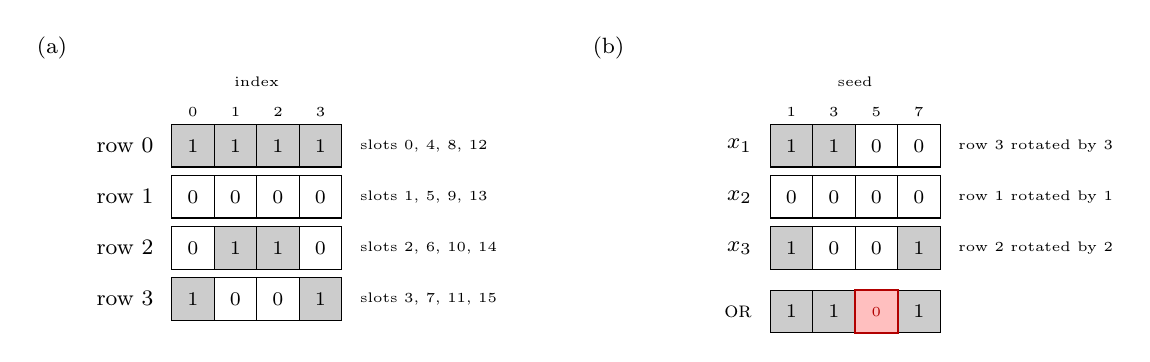
\begin{tikzpicture}[x=5.4mm,y=5.4mm,font=\footnotesize,>={Latex[length=1.6mm]}]
\def\bits#1#2#3#4{% name, x, y, bits
  \node[left] at (#2-.2,#3+.5) {#1};
  \foreach \v [count=\d from 0] in {#4} {
    \ifnum\v=1 \fill[gray!40] (#2+\d,#3) rectangle ++(1,1); \fi
    \draw (#2+\d,#3) rectangle ++(1,1);
    \node[font=\scriptsize] at (#2+\d+.5,#3+.5) {$\v$};
  }}
% (a) The rows of the set of used slots of Figure 1
\node[anchor=west] at (-3.4,6.4) {(a)};
\node[font=\tiny] at (2,5.6) {index};
\foreach \d in {0,...,3} \node[font=\tiny] at (\d+.5,4.9) {$\d$};
\bits{row $0$}{0}{3.6}{1,1,1,1}
\bits{row $1$}{0}{2.4}{0,0,0,0}
\bits{row $2$}{0}{1.2}{0,1,1,0}
\bits{row $3$}{0}{0}{1,0,0,1}
\foreach \y/\l in {3.6/{0, 4, 8, 12},2.4/{1, 5, 9, 13},1.2/{2, 6, 10, 14},0/{3, 7, 11, 15}}
  \node[right,font=\tiny] at (4.2,\y+.5) {slots \l};
% (b) Pattern 1: rings rotated by the index of the base position
\begin{scope}[xshift=76mm]
\node[anchor=west] at (-4.4,6.4) {(b)};
\node[font=\tiny] at (2,5.6) {seed};
\foreach \s [count=\d from 0] in {1,3,5,7} \node[font=\tiny] at (\d+.5,4.9) {$\s$};
\bits{$x_1$}{0}{3.6}{1,1,0,0}
\bits{$x_2$}{0}{2.4}{0,0,0,0}
\bits{$x_3$}{0}{1.2}{1,0,0,1}
\bits{\textsc{or}}{0}{-.3}{1,1,0,1}
\draw[red!70!black,thick,fill=red!25] (2,-.3) rectangle ++(1,1)
  node[midway,font=\tiny,text=red!70!black] {$0$};
\foreach \y/\l in {3.6/{row $3$ rotated by $3$},2.4/{row $1$ rotated by $1$},1.2/{row $2$ rotated by $2$}}
  \node[right,font=\tiny] at (4.2,\y+.5) {\l};
\end{scope}
\end{tikzpicture}
\caption{\label{fig:search}Finding the free rotations of pattern $1$ for the
bucket of Figure~\ref{fig:placement}. (a) The set of used
slots is stored by residue classes modulo the stride $T=4$: bit $q$ of row
$\varrho$ records whether slot $qT+\varrho$ is used. (b) The bits of the ring
of a key form a row (in general, a block of consecutive bits of a row), and
the rotations go through them cyclically, starting from the index of the base position of
the key: for example, the base position of $x_1$ is slot $15$ (seed $1$),
which has index $3$ in row $3$. The bits of the rings, rotated by these
indices, are combined by a bitwise \textsc{or}: the zeros of the result are
the free rotations (here, only rotation $2$, that is, seed $5$).}
\end{figure}

\paragraph{Search.}
In a bitmap of the used slots, the bits of the slots of a ring would be $T$
bits apart. We make them adjacent by storing the set of used slots by residue
classes modulo $T$, that is, as $T$ \emph{rows} in which bit $q$ of row
$\varrho$ records whether slot $qT+\varrho$ is used. All the slots of a ring
have the same residue modulo $T$ (wrapping around the end of a slice does not
change it, as $T$ divides $L$), so the bits of the ring of a key are a block
of $L/T$ consecutive bits of a row, and rotation $j$ maps the key to the bit
of the block of index $(x+j)\bmod(L/T)$, where $x$ is the index in the block
of the bit of its base position. Thus, rotating the block cyclically so that
its bit $x$ becomes bit $0$ we obtain a block whose bit $j$ tells whether
rotation $j$ maps the key to a used slot, and combining these blocks for all
the keys of the bucket by a bitwise \textsc{or} we obtain a block whose zeros
are the \emph{free} rotations, which map no key to a used slot
(Figure~\ref{fig:search}). A free rotation $j$ yields the feasible seed $jR+r$
unless two keys of the bucket are mapped to the same slot, which is rare. For
$S=8$ and $R=4$ a ring has $2^{S-\rho}=64$ slots whatever the slice length, so
its bits fill a word: each
pattern requires just reading and rotating a word for each key. Note that
rotation $0$ of pattern $0$ (seed $0$) is not available.

Among the free rotations of all patterns we choose, as in \PHast, the one
minimizing the sum of the slots of the keys. For a bucket of size $k$, the sum for rotation $j$ of a
pattern is the sum for rotation $0$ plus $kjT$,
minus $L$ for each key that has wrapped around the end of its slice, that is,
for each key such that $x+j\geq L/T$. To count such keys we pack the indices
$x$ of the base positions of the keys of the bucket into fields of a word
that are large enough to contain the sum of two indices (for $S=8$ and $R=4$, eight fields of eight bits):
after adding $j$ to all fields with a single addition, the bit of weight $L/T$
of each field tells whether the corresponding key has wrapped around, and
counting such bits gives the number of keys that have wrapped around.
Evaluating a seed thus requires a number of operations that does not depend
on the size of the bucket (for buckets with at most eight keys, in the case
above), and since buckets have usually just a few free rotations (on average
$4.5$ with $\lambda=5$) we evaluate all of them, with a single loop over the
zeros of the blocks of all patterns that contains no other branch. When there
are many free rotations (e.g., at the beginning of a sweep) we use instead the
fact that in a pattern the sum increases with the rotation, except at the
rotations at which some key wraps around: thus, we need to consider only the
first free rotation and, for each key, the first free rotation not smaller
than the one at which the key wraps around, that is, at most $k+1$ candidates
per pattern. Finally, when marking the slots of the best free rotation as used
we check that no two keys of the bucket are mapped to the same slot, and
otherwise we move to the next best one.

\paragraph{Grouping and scheduling.}
The sweep needs the hashes of the keys of each bucket, but in no particular
order, and we do not want to keep more than one copy of them. Thus, we
distribute them into at most $256$ \emph{parts}, each made of a power-of-two
number of consecutive buckets: each thread computes the hashes of a chunk of
the keys, and appends each hash to the \emph{region} associated with the
chunk and with the part of the hash, recording the part in a byte; the hashes
in a region are thus in the order of the keys. Regions are sized before
computing the hashes, assuming that hashes are uniform, with a slack of six
standard deviations: the few hashes that do not fit their region, if any, are
kept separately. A part is distributed into buckets only when a sweep needs
it, into a buffer of the sweep (the part is distributed first into smaller
parts that fit the cache, and then each smaller part into its buckets), so
regions are never modified. After the sweep, the keys of bumped buckets, which
must be passed to the next level, are found by walking again the keys of each
chunk in order: the byte of a key gives its part, its hash is the next unread
hash of the region of the chunk for that part, and a bit vector with a bit
per bucket tells whether the bucket of the hash has been bumped. Writing to
at most $256$ regions at a time and working on smaller parts of about
$150$\,KB is
efficient on any current architecture, and the construction needs, besides
the hashes, just a byte per key: about $11$ bytes per key overall.

The priority of a bucket has the same form as in \PHast: a weight depending
on the size of the bucket (we use the weights of \PHastP with wrapping,
extrapolated linearly beyond size $7$), minus $1024$ times the index of the
bucket. Since buckets enter the window of the sweep in order of index, the
buckets of each size in the window form a queue, and the bucket with the
highest priority is the first bucket of one of the queues. Instead of a
priority queue we keep a queue for each size: extracting the next bucket
requires scanning the first elements of a few queues, and adding a bucket
takes constant time. Finally, the set of used slots of the level, which is
needed to build the Elias--Fano sequence remapping the outputs of the
following levels, is a byproduct of the sweep: the sweep keeps in a cyclic
buffer only the bits of the slots that the buckets still to be placed can
reach, and copies the bits of the slots that are no longer reachable to the
bitmap of the level when their space in the buffer is recycled.

\paragraph{Slice length.}
The slice length of a level with output range $m$ is the smallest power of two
larger than $m/2$, up to a maximum, which is a parameter: we use $L=1024$ for
$S=8$ and $L=2048$ for $S=10$, as \PHastP with wrapping does. The slices of
small levels can thus have fewer slots than there are seeds, that is,
$\ell<S$: in this case the slot of a key is
$\sigma(h)+\bigl(\omega_r(o)+s\bigr)\bmod L$, so the stride is $R$, rings
have $L/R$ slots (a single slot if $L<R$), and rotations $j$ and $j'$ map the
keys of a bucket to the same slots whenever $L$ divides $(j-j')R$.

\paragraph{Levels.}
Levels after the first use the same scheme with range equal to their number of
keys, and an Elias--Fano sequence maps their outputs to the holes of the first
level. A bumped key is hashed again just once, with a different hash seed: if $h'$
is this second hash, the value playing the role of $h$ at level $i>1$ is
\[
\hi\bigl((h\oplus z_i)(h'\oplus c)\bigr)\oplus\operatorname{lo}\bigl((h\oplus z_i)(h'\oplus c)\bigr),
\]
where $z_i$ is a \emph{salt} associated with the level and $c$ is a constant.
Thus, the levels after the first depend only on $h$ and $h'$: once $h'$ has
been computed the key is no longer needed, and the code accessing the
following levels, which takes just two integers, can be kept separate from
that accessing the first level.

\paragraph{Colliding hashes.}
Keys with the same $64$-bit hash at the first level have the same slice and
the same offsets in all patterns, so they collide for every seed and their
bucket is bumped; at the following levels the values playing the role of $h$
depend also on the second hash, and thus they are separated. Since about $n^2/2^{65}$ pairs of
keys have the same hash (about three for $n=10^{10}$), the keys bumped in this
way are negligible with respect to the $\beta n$ keys that are bumped anyway.
Hence, $64$-bit hashes are sufficient for any number of keys. Construction would fail only if two keys had the same pair of
hashes, which happens in practice only for duplicate keys. Since duplicate
keys are always bumped from the first level, to report them we examine the
buckets of the following levels: keys of a bucket with the same value are
hashed with a third hash seed, and keys whose hashes coincide again are considered
duplicates.

\paragraph{Last level.}
When at most $4096$ keys are left, a last level with $k$ keys uses the same
placement scheme with a range of $\lfloor 5k/4\rfloor+16$ slots, expected
bucket size $\min(\lambda,3)$, and
no bumping, changing the salt (and, every eight
attempts, enlarging the range) in the unlikely case of failure.

\paragraph{Parallel construction.}
As in \PHast, buckets are split into chunks separated by gaps of
\[
\left\lfloor \frac{LB}{m-L+1}\right\rfloor+1
\]
buckets: the slice of bucket $b$ starts at about $b(m-L+1)/B$, and the slot
of a key lies at most $L-1$ slots after the start of its slice, so
(considering the rounding of slice starts) the keys of different chunks
cannot reach the same slots. Chunks are swept in parallel, and then all gaps
are swept in parallel, each with a new sweep in which the slots used by the
keys of the neighboring chunks (on both sides) are marked as used.

\section{Differences from \PHast and \PHastP}
\label{sec:differences}

In \PHast~\cite{BeSPHast}, in its variant \PHastP, and in \PHastR the bucket
of a key with hash $h$ is $\hi(hB)$, and the seed $s$ of the bucket places the
key at $\sigma(h)+p(s,h)$, where $\sigma(h)$ is the start of its slice: the
three structures differ mainly in the in-slice position $p(s,h)$. In \PHast,
$p(s,h)$ is a pseudorandom function, so finding the best seed requires trying
all seeds. \PHastP uses instead the additive placement $p(s,h)=(h\bmod
L)+s-1$, so that feasible seeds can be found by combining windows of the
bitmap of used slots, but it needs more space than \PHast; \PHastP
\emph{with wrapping} uses $p(s,h)=(h+\delta s)\bmod L$ for a small multiplier
$\delta$, so that keys do not leave their slice, and needs less space than
\PHastP without wrapping, but it is slower to build. In \PHastR, $p(s,h)=\bigl(\omega_r(o)+(s\ll(\ell-S))\bigr)\bmod L$,
where $r=s\bmod R$ and $o=\operatorname{lo}(hB)$.

\paragraph{Additive placement is rigid.}
As in \PHastR, the first level of \PHastP has output range $m=n$, so its holes
are exactly its bumped keys, and by~(\ref{eq:space}) its excess space comes
from bumping. Additive placement, however, moves all the keys of a bucket by
the same amount: two keys of a bucket that collide for one seed, which
happens with probability about $k(k-1)/(2L)$ for a bucket of size $k$,
collide for every seed. Wrapping does not change the picture, as two such keys move
together around their slices, and collide for all seeds but the few for
which exactly one of them has wrapped. Inspecting the first level of the
reference implementation, we found that these self-collisions cause a large
part of the bumping (almost $40\%$ with wrapping). Moreover, consecutive
seeds move a fixed arrangement of the keys of a bucket, and are thus strongly
correlated attempts at placing it, and the excess space cannot be
recovered by compressing the seeds, which are almost incompressible.

\paragraph{Patterns instead of a rigid pattern.}
In \PHastR the seed first chooses among $R$ patterns, whose offsets come from
disjoint blocks of bits of $o$, and then a rotation, which moves the keys
along their rings. Since self-collisions happen independently in each
pattern, buckets with a self-collision in every pattern are negligible
already for $R=2$ (in Figure~\ref{fig:placement}, the keys $x_1$ and $x_2$
would collide for all seeds in \PHastP, but in \PHastR they collide only for
the seeds choosing pattern~$0$), and different patterns are (almost)
independent attempts at placing a bucket. Queries need just two shifts
more than in \PHastP with wrapping, and wrapping does not complicate the
search: in \PHastP with wrapping the range of seeds must be split at the
points at which some key wraps, and with $\delta>1$ only one bit out of
$\delta$ of each window of the bitmap is meaningful, whereas in \PHastR the
bits recording the slots of a key for the rotations of a pattern are adjacent
bits of a row, and wrapping is taken care of by the rotation of the block.

\paragraph{Construction.}
The construction of \PHastR differs from that of the reference implementation
also in several engineering aspects (Section~\ref{sec:phastr}): hashes are
distributed into parts rather than sorted, the priority queue is replaced by
a queue for each bucket size, bumped keys are hashed again just once rather
than at each level, the last level uses the same scheme as the other levels
rather than the pseudorandom placement of \PHast, and the gaps between the
chunks of a parallel construction are swept in parallel rather than
serially. Slice lengths and bucket priorities are those of \PHastP with
wrapping, but the expected bucket size is smaller.

\section{Experiments}
\label{sec:experiments}

We ran all experiments on an Amazon EC2 \texttt{c7i.metal-24xl} instance
(one Intel Xeon Platinum 8488C with 48 cores, 105\,MB of L3 cache and
192\,GiB of RAM), compiling with Rust 1.99 at optimization level 3 with thin
link-time optimization. Keys are distinct 64-bit integers. The reference
implementation is the \texttt{ph} crate by Beling (\texttt{Function2} with
the \texttt{ShiftOnly}, \texttt{ShiftOnlyWrapped<$\delta$>} and
\texttt{SeedOnly} seed choosers for \PHastP, \PHastP with wrapping and \PHast,
respectively). To make query times comparable we fed both implementations the
same hash function, GxHash with a hash seed, as in the experiments of the \PHast
paper. Construction times are single-threaded unless otherwise noted and
include hashing; query times are medians over nine rounds of $2\cdot10^6$
queries of consecutive keys of the set, and the rounds of the different
structures are interleaved. Since all structures hash the key first, their
memory accesses are random anyway: reading the keys in order avoids adding to
every query the same cache miss on the array of keys. \PHastR uses $R=4$ patterns, with byte seeds for $S=8$ and
bit-packed seeds read without alignment for $S=10$.

\begin{table}[t]
\centering
\caption{Comparison on $10^7$ keys (single-threaded construction).}
\label{tab:1e7}
\small
\begin{tabular}{llrrr}
\toprule
Method & Configuration & bits/key & build [ns/key] & query [ns] \\
\midrule
\PHastP & $S=8$, $\lambda=5.25$ & 2.116 & 52 & 7.6 \\
\PHastP wrap $\delta=1$ & $S=8$, $\lambda=5.25$ & 2.096 & 65 & 7.4 \\
\PHastP wrap $\delta=2$ & $S=8$, $\lambda=5$ & 2.013 & 76 & 6.0 \\
\PHastP wrap $\delta=3$ & $S=8$, $\lambda=5$ & 1.970 & 86 & 5.9 \\
\PHast & $S=8$, $\lambda=4.5$ & 1.922 & 641 & 4.8 \\
\addlinespace
\PHastR & $S=8$, $L=1024$, $\lambda=4.5$ & 1.929 & 44 & 4.6 \\
\PHastR & $S=8$, $L=1024$, $\lambda=4.75$ & 1.921 & 43 & 5.1 \\
\PHastR & $S=8$, $L=1024$, $\lambda=5$ & 1.925 & 43 & 5.7 \\
\midrule
\PHastP & $S=10$, $\lambda=5.15$ & 2.085 & 54 & 6.5 \\
\PHastP wrap $\delta=1$ & $S=10$, $\lambda=6.2$ & 1.905 & 78 & 7.0 \\
\PHastP wrap $\delta=2$ & $S=10$, $\lambda=5.9$ & 1.883 & 103 & 6.3 \\
\PHastP wrap $\delta=3$ & $S=10$, $\lambda=6$ & 1.872 & 133 & 6.6 \\
\PHast & $S=10$, $\lambda=6.05$ & 1.854 & 1829 & 7.0 \\
\addlinespace
\PHastR & $S=10$, $L=2048$, $\lambda=5.75$ & 1.858 & 85 & 5.5 \\
\PHastR & $S=10$, $L=2048$, $\lambda=6$ & 1.852 & 81 & 5.9 \\
\PHastR & $S=10$, $L=2048$, $\lambda=6.25$ & 1.857 & 80 & 6.3 \\
\bottomrule
\end{tabular}
\end{table}

Table~\ref{tab:1e7} shows the results on $10^7$ keys, a size at which the
structures fit in the cache. With 8-bit seeds and
the suggested expected bucket size $\lambda=4.5$, \PHastR uses $0.04$ bits
per key less than the best variant of \PHastP with wrapping, and it is built
in half the time (it is faster to build even than \PHastP without wrapping).
Its queries are faster than those of all variants of \PHastP ($22\%$ faster
than those of the variant using the least space), and slightly faster than
those of \PHast, which uses $0.4\%$ less space but takes fifteen times as
long to build. Queries are fast because \PHastR bumps few keys: just $1.5\%$
of the keys from the first level, against the $4.3\%$ of \PHastP with
wrapping and $\delta=3$, and queries for bumped keys are much slower than the
others. The expected bucket size thus trades space for query time: with
$\lambda=4.75$ \PHastR bumps $2.5\%$ of the keys, and it has the space of
\PHast and slightly slower queries; with $\lambda=5$ it bumps $3.7\%$ of the
keys, and its queries are still slightly faster than those of \PHastP with
wrapping and $\delta=3$. With 10-bit seeds and $\lambda=5.75$ \PHastR uses
less space than all variants of \PHastP, and it is built in $64\%$ of the
time of \PHastP with wrapping and $\delta=3$; with $\lambda=6$ it uses
slightly less space than \PHast. In both cases its queries are faster than
those of all the other structures with 10-bit seeds.

\begin{table}[t]
\centering
\caption{Comparison on $10^8$ keys, with single-threaded and 8-threaded
construction.}
\label{tab:1e8}
\small
\begin{tabular}{llrrrr}
\toprule
& & & \multicolumn{2}{c}{build [ns/key]} & \\
\cmidrule(lr){4-5}
Method & Configuration & bits/key & 1 thread & 8 threads & query [ns] \\
\midrule
\PHastP & $S=8$, $\lambda=5.25$ & 2.115 & 58 & 11.6 & 16.2 \\
\PHastP wrap $\delta=3$ & $S=8$, $\lambda=5$ & 1.968 & 93 & 17.1 & 13.5 \\
\PHast & $S=8$, $\lambda=4.5$ & 1.921 & 646 & 85.6 & 11.5 \\
\addlinespace
\PHastR & $S=8$, $L=1024$, $\lambda=4.5$ & 1.927 & 50 & 7.6 & 11.0 \\
\PHastR & $S=8$, $L=1024$, $\lambda=4.75$ & 1.919 & 50 & 7.8 & 11.8 \\
\PHastR & $S=8$, $L=1024$, $\lambda=5$ & 1.924 & 49 & 8.1 & 12.8 \\
\midrule
\PHastP wrap $\delta=3$ & $S=10$, $\lambda=6$ & 1.869 & 139 & 22.5 & 14.9 \\
\addlinespace
\PHastR & $S=10$, $L=2048$, $\lambda=5.75$ & 1.854 & 90 & 12.7 & 12.7 \\
\PHastR & $S=10$, $L=2048$, $\lambda=6$ & 1.849 & 88 & 12.6 & 13.4 \\
\bottomrule
\end{tabular}
\end{table}

Table~\ref{tab:1e8} shows that the picture does not change on $10^8$ keys,
where queries are dominated by cache misses: with 8-bit seeds and
$\lambda=4.5$ \PHastR is built in $54\%$ of the time of \PHastP with
wrapping, and its queries are $19\%$ faster; they are also slightly faster
than those of \PHast. With 8 threads \PHastR is built in $44\%$ of the time of
\PHastP with wrapping when seeds have 8 bits, and in $56\%$ of the time when
they have 10 bits.

\subsection{Large Key Sets}
\label{sec:large}

\begin{table}[t]
\centering
\caption{Comparison on $10^9$ keys, with single-threaded and 8-threaded
construction.}
\label{tab:1e9}
\small
\begin{tabular}{llrrrr}
\toprule
& & & \multicolumn{2}{c}{build [ns/key]} & \\
\cmidrule(lr){4-5}
Method & Configuration & bits/key & 1 thread & 8 threads & query [ns] \\
\midrule
\PHastP & $S=8$, $\lambda=5.25$ & 2.115 & 64 & 12.6 & 32.3 \\
\PHastP wrap $\delta=3$ & $S=8$, $\lambda=5$ & 1.968 & 98 & 18.0 & 26.2 \\
\PHast & $S=8$, $\lambda=4.5$ & 1.920 & 652 & 86.3 & 21.6 \\
\addlinespace
\PHastR & $S=8$, $L=1024$, $\lambda=4.5$ & 1.927 & 54 & 8.2 & 20.4 \\
\PHastR & $S=8$, $L=1024$, $\lambda=4.75$ & 1.919 & 53 & 8.8 & 22.5 \\
\PHastR & $S=8$, $L=1024$, $\lambda=5$ & 1.924 & 53 & 8.6 & 25.0 \\
\midrule
\PHastP wrap $\delta=3$ & $S=10$, $\lambda=6$ & 1.869 & 148 & 24.0 & 28.5 \\
\addlinespace
\PHastR & $S=10$, $L=2048$, $\lambda=5.75$ & 1.854 & 93 & 13.6 & 24.6 \\
\PHastR & $S=10$, $L=2048$, $\lambda=6$ & 1.848 & 91 & 13.5 & 26.3 \\
\bottomrule
\end{tabular}
\end{table}

Table~\ref{tab:1e9} reports the results on $10^9$ keys. Space does not depend
on the number of keys, and the relative performance of the structures is the
same as on smaller key sets: with 8-bit seeds \PHastR is built in $55\%$ of
the time of \PHastP with wrapping with one thread, and in less than half the
time with eight, its queries are $22\%$ faster, and they are slightly faster
than those of \PHast. At this scale, however, the cost of bumped keys becomes
more visible, and we used it to choose the suggested expected bucket size.

\begin{table}[t]
\centering
\caption{Query time in nanoseconds for the keys of the first level
(``first'') and for all keys; the second column is the percentage of keys
bumped from the first level.}
\label{tab:split}
\small
\begin{tabular}{lrrrrrrr}
\toprule
& & \multicolumn{2}{c}{$10^7$ keys} & \multicolumn{2}{c}{$10^8$ keys} & \multicolumn{2}{c}{$10^9$ keys} \\
\cmidrule(lr){3-4}\cmidrule(lr){5-6}\cmidrule(lr){7-8}
Structure & bumped & first & all & first & all & first & all \\
\midrule
\PHastP wrap $\delta=3$, $\lambda=5$ & 4.3 & 3.8 & 5.9 & 5.8 & 11.1 & 14.8 & 24.9 \\
\PHast, $\lambda=4.5$ & 1.4 & 4.1 & 4.7 & 5.8 & 9.0 & 15.6 & 20.9 \\
\PHastR, $\lambda=4.5$ & 1.5 & 3.8 & 4.5 & 5.7 & 8.5 & 14.7 & 19.7 \\
\PHastR, $\lambda=4.75$ & 2.5 & 3.8 & 5.0 & 5.7 & 9.3 & 14.5 & 21.5 \\
\bottomrule
\end{tabular}
\end{table}

\begin{figure}[tp]
\centering
% Generated by lab/results/paper/plot_pareto.py c7i/run.csv
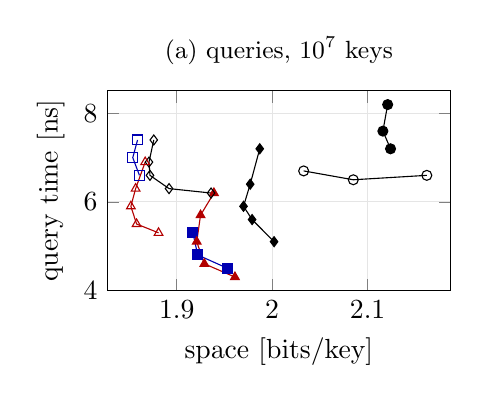
\begin{tikzpicture}
\begin{axis}[
  width=0.49\textwidth, height=0.34\textwidth, title style={font=\small},
  title={(a) queries, $10^{7}$ keys},
  xlabel={space [bits/key]}, ylabel={query time [ns]}, enlargelimits=0.08,
  grid=major, grid style={gray!20}, legend to name=leg:pareto, legend columns=4, legend cell align=left, legend style={font=\small, /tikz/every even column/.append style={column sep=0.5em}}]
\addplot[mark=*, color=black, mark size=1.8pt] coordinates { (2.124,7.2) (2.116,7.6) (2.121,8.2) };
\addplot[mark=diamond*, color=black, mark size=1.8pt] coordinates { (2.002,5.1) (1.979,5.6) (1.970,5.9) (1.977,6.4) (1.987,7.2) };
\addplot[mark=square*, color=blue!70!black, mark size=1.8pt] coordinates { (1.953,4.5) (1.922,4.8) (1.917,5.3) };
\addplot[mark=triangle*, color=red!70!black, mark size=1.8pt] coordinates { (1.961,4.3) (1.929,4.6) (1.921,5.1) (1.925,5.7) (1.939,6.2) };
\addplot[mark=o, color=black, mark size=1.8pt] coordinates { (2.162,6.6) (2.085,6.5) (2.033,6.7) };
\addplot[mark=diamond, color=black, mark size=1.8pt] coordinates { (1.936,6.2) (1.892,6.3) (1.872,6.6) (1.871,6.9) (1.876,7.4) };
\addplot[mark=square, color=blue!70!black, mark size=1.8pt] coordinates { (1.861,6.6) (1.854,7.0) (1.859,7.4) };
\addplot[mark=triangle, color=red!70!black, mark size=1.8pt] coordinates { (1.881,5.3) (1.858,5.5) (1.852,5.9) (1.857,6.3) (1.867,6.9) };
\legend{\PHastP ($S=8$), \PHastP wrap $\delta=3$ ($S=8$), \PHast ($S=8$), \PHastR ($S=8$), \PHastP ($S=10$), \PHastP wrap $\delta=3$ ($S=10$), \PHast ($S=10$), \PHastR ($S=10$)}
\end{axis}
\end{tikzpicture}%
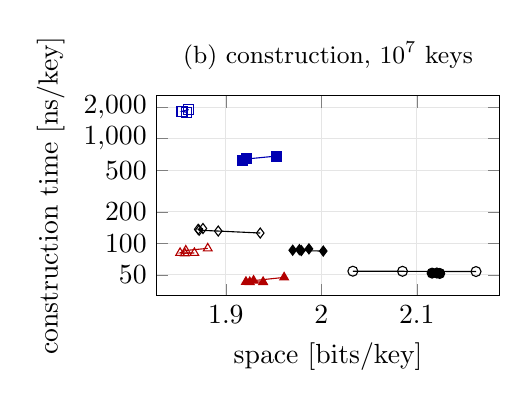
\begin{tikzpicture}
\begin{axis}[
  width=0.49\textwidth, height=0.34\textwidth, title style={font=\small},
  title={(b) construction, $10^{7}$ keys},
  xlabel={space [bits/key]}, ylabel={construction time [ns/key]}, ymode=log, log ticks with fixed point, ytick={20,50,100,200,500,1000,2000}, enlargelimits=0.08,
  grid=major, grid style={gray!20}]
\addplot[mark=*, color=black, mark size=1.8pt] coordinates { (2.124,51.5) (2.116,51.9) (2.121,52.0) };
\addplot[mark=diamond*, color=black, mark size=1.8pt] coordinates { (2.002,84.3) (1.979,85.2) (1.970,85.9) (1.977,87.0) (1.987,88.5) };
\addplot[mark=square*, color=blue!70!black, mark size=1.8pt] coordinates { (1.953,682.8) (1.922,640.7) (1.917,614.2) };
\addplot[mark=triangle*, color=red!70!black, mark size=1.8pt] coordinates { (1.961,47.2) (1.929,44.0) (1.921,42.8) (1.925,42.6) (1.939,42.7) };
\addplot[mark=o, color=black, mark size=1.8pt] coordinates { (2.162,53.7) (2.085,54.0) (2.033,54.1) };
\addplot[mark=diamond, color=black, mark size=1.8pt] coordinates { (1.936,125.4) (1.892,131.0) (1.872,133.3) (1.871,136.2) (1.876,138.6) };
\addplot[mark=square, color=blue!70!black, mark size=1.8pt] coordinates { (1.861,1900.4) (1.854,1829.4) (1.859,1785.8) };
\addplot[mark=triangle, color=red!70!black, mark size=1.8pt] coordinates { (1.881,89.5) (1.858,85.4) (1.852,81.0) (1.857,80.4) (1.867,80.9) };
\end{axis}
\end{tikzpicture}\\[1ex]
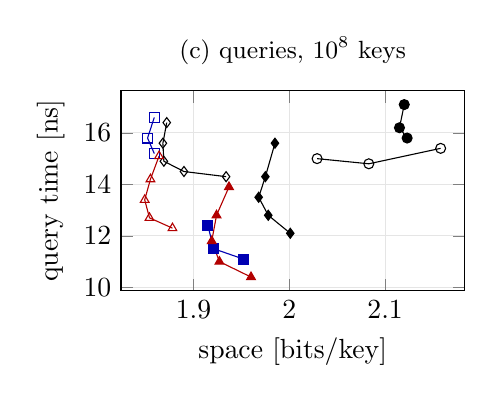
\begin{tikzpicture}
\begin{axis}[
  width=0.49\textwidth, height=0.34\textwidth, title style={font=\small},
  title={(c) queries, $10^{8}$ keys},
  xlabel={space [bits/key]}, ylabel={query time [ns]}, enlargelimits=0.08,
  grid=major, grid style={gray!20}]
\addplot[mark=*, color=black, mark size=1.8pt] coordinates { (2.123,15.8) (2.115,16.2) (2.120,17.1) };
\addplot[mark=diamond*, color=black, mark size=1.8pt] coordinates { (2.001,12.1) (1.978,12.8) (1.968,13.5) (1.975,14.3) (1.985,15.6) };
\addplot[mark=square*, color=blue!70!black, mark size=1.8pt] coordinates { (1.952,11.1) (1.921,11.5) (1.915,12.4) };
\addplot[mark=triangle*, color=red!70!black, mark size=1.8pt] coordinates { (1.960,10.4) (1.927,11.0) (1.919,11.8) (1.924,12.8) (1.937,13.9) };
\addplot[mark=o, color=black, mark size=1.8pt] coordinates { (2.158,15.4) (2.083,14.8) (2.029,15.0) };
\addplot[mark=diamond, color=black, mark size=1.8pt] coordinates { (1.934,14.3) (1.890,14.5) (1.869,14.9) (1.868,15.6) (1.872,16.4) };
\addplot[mark=square, color=blue!70!black, mark size=1.8pt] coordinates { (1.859,15.2) (1.852,15.8) (1.859,16.6) };
\addplot[mark=triangle, color=red!70!black, mark size=1.8pt] coordinates { (1.878,12.3) (1.854,12.7) (1.849,13.4) (1.855,14.2) (1.864,15.1) };
\end{axis}
\end{tikzpicture}%
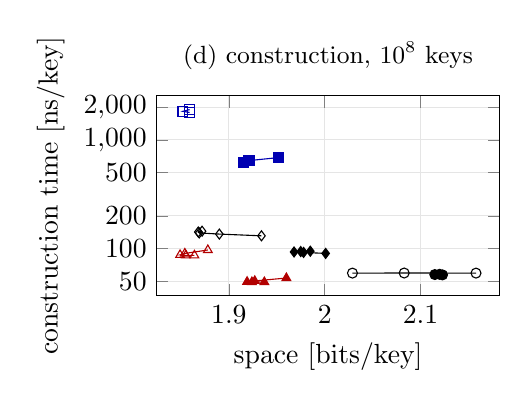
\begin{tikzpicture}
\begin{axis}[
  width=0.49\textwidth, height=0.34\textwidth, title style={font=\small},
  title={(d) construction, $10^{8}$ keys},
  xlabel={space [bits/key]}, ylabel={construction time [ns/key]}, ymode=log, log ticks with fixed point, ytick={20,50,100,200,500,1000,2000}, enlargelimits=0.08,
  grid=major, grid style={gray!20}]
\addplot[mark=*, color=black, mark size=1.8pt] coordinates { (2.123,57.3) (2.115,57.7) (2.120,58.0) };
\addplot[mark=diamond*, color=black, mark size=1.8pt] coordinates { (2.001,90.3) (1.978,92.2) (1.968,93.1) (1.975,93.9) (1.985,94.6) };
\addplot[mark=square*, color=blue!70!black, mark size=1.8pt] coordinates { (1.952,688.1) (1.921,645.6) (1.915,618.9) };
\addplot[mark=triangle*, color=red!70!black, mark size=1.8pt] coordinates { (1.960,53.6) (1.927,50.4) (1.919,49.5) (1.924,49.2) (1.937,49.2) };
\addplot[mark=o, color=black, mark size=1.8pt] coordinates { (2.158,59.5) (2.083,59.6) (2.029,59.5) };
\addplot[mark=diamond, color=black, mark size=1.8pt] coordinates { (1.934,131.1) (1.890,136.0) (1.869,139.4) (1.868,142.1) (1.872,144.6) };
\addplot[mark=square, color=blue!70!black, mark size=1.8pt] coordinates { (1.859,1902.2) (1.852,1833.3) (1.859,1788.3) };
\addplot[mark=triangle, color=red!70!black, mark size=1.8pt] coordinates { (1.878,97.1) (1.854,90.2) (1.849,87.5) (1.855,86.6) (1.864,86.7) };
\end{axis}
\end{tikzpicture}\\[1ex]
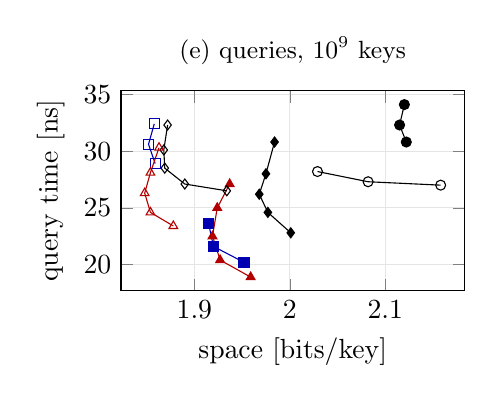
\begin{tikzpicture}
\begin{axis}[
  width=0.49\textwidth, height=0.34\textwidth, title style={font=\small},
  title={(e) queries, $10^{9}$ keys},
  xlabel={space [bits/key]}, ylabel={query time [ns]}, enlargelimits=0.08,
  grid=major, grid style={gray!20}]
\addplot[mark=*, color=black, mark size=1.8pt] coordinates { (2.122,30.8) (2.115,32.3) (2.120,34.1) };
\addplot[mark=diamond*, color=black, mark size=1.8pt] coordinates { (2.001,22.8) (1.977,24.6) (1.968,26.2) (1.975,28.0) (1.984,30.8) };
\addplot[mark=square*, color=blue!70!black, mark size=1.8pt] coordinates { (1.952,20.2) (1.920,21.6) (1.915,23.6) };
\addplot[mark=triangle*, color=red!70!black, mark size=1.8pt] coordinates { (1.959,18.9) (1.927,20.4) (1.919,22.5) (1.924,25.0) (1.937,27.1) };
\addplot[mark=o, color=black, mark size=1.8pt] coordinates { (2.158,27.0) (2.082,27.3) (2.029,28.2) };
\addplot[mark=diamond, color=black, mark size=1.8pt] coordinates { (1.934,26.5) (1.890,27.1) (1.869,28.5) (1.868,30.1) (1.872,32.3) };
\addplot[mark=square, color=blue!70!black, mark size=1.8pt] coordinates { (1.859,28.9) (1.852,30.6) (1.858,32.4) };
\addplot[mark=triangle, color=red!70!black, mark size=1.8pt] coordinates { (1.878,23.4) (1.854,24.6) (1.848,26.3) (1.854,28.1) (1.863,30.3) };
\end{axis}
\end{tikzpicture}%
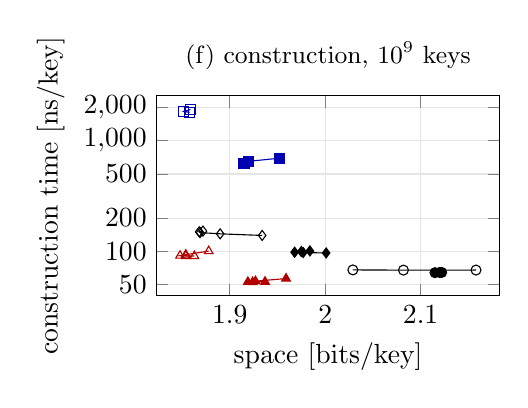
\begin{tikzpicture}
\begin{axis}[
  width=0.49\textwidth, height=0.34\textwidth, title style={font=\small},
  title={(f) construction, $10^{9}$ keys},
  xlabel={space [bits/key]}, ylabel={construction time [ns/key]}, ymode=log, log ticks with fixed point, ytick={20,50,100,200,500,1000,2000}, enlargelimits=0.08,
  grid=major, grid style={gray!20}]
\addplot[mark=*, color=black, mark size=1.8pt] coordinates { (2.122,64.5) (2.115,64.2) (2.120,64.5) };
\addplot[mark=diamond*, color=black, mark size=1.8pt] coordinates { (2.001,96.7) (1.977,97.6) (1.968,98.3) (1.975,99.6) (1.984,100.9) };
\addplot[mark=square*, color=blue!70!black, mark size=1.8pt] coordinates { (1.952,694.4) (1.920,651.7) (1.915,624.9) };
\addplot[mark=triangle*, color=red!70!black, mark size=1.8pt] coordinates { (1.959,56.8) (1.927,53.8) (1.919,53.0) (1.924,52.8) (1.937,53.2) };
\addplot[mark=o, color=black, mark size=1.8pt] coordinates { (2.158,67.8) (2.082,67.7) (2.029,68.0) };
\addplot[mark=diamond, color=black, mark size=1.8pt] coordinates { (1.934,139.3) (1.890,144.0) (1.869,147.8) (1.868,150.1) (1.872,152.5) };
\addplot[mark=square, color=blue!70!black, mark size=1.8pt] coordinates { (1.859,1910.4) (1.852,1841.6) (1.858,1797.0) };
\addplot[mark=triangle, color=red!70!black, mark size=1.8pt] coordinates { (1.878,100.5) (1.854,93.4) (1.848,91.4) (1.854,90.9) (1.863,90.8) };
\end{axis}
\end{tikzpicture}\\[1ex]
\ref{leg:pareto}
\caption{Space versus query time (left) and single-threaded construction time
(right) on $10^7$, $10^8$ and $10^9$ keys (top to bottom) as the expected
bucket size varies in steps of $0.25$ around the configurations of
Table~\ref{tab:1e7}: from $4.25$ to $5.25$ (\PHastR), from $4.5$ to $5.5$
(\PHastP wrap $\delta=3$) and by $0.25$ on each side (the others) with 8-bit
seeds, and from $5.5$ to $6.5$ (\PHastR and \PHastP wrap $\delta=3$) and by
$0.25$ on each side (the others) with 10-bit seeds; the configurations of
each structure are joined in order of expected bucket size.}
\label{fig:pareto}
\end{figure}

\paragraph{Trade-offs.}
Figure~\ref{fig:pareto} shows what happens when the expected bucket size
varies around the configurations of the tables. Space has a minimum, query
time grows with $\lambda$, as more keys are bumped, and construction time
varies by less than $15\%$. The curves of \PHast and \PHastR are close in
space, but their construction times differ by more than a factor of ten; with
10-bit seeds
\PHastR has also faster queries. The curves of \PHastP with wrapping are to
the right of both. Considering the three dimensions at once,
on $10^9$ keys no configuration of \PHastP, with or without wrapping, is
Pareto-optimal: each is dominated by a configuration of \PHastR with less
space, faster queries and a faster construction. The only other
configurations that are not dominated are those of \PHast with $8$-bit seeds
and $\lambda=4.25$ and $\lambda=4.5$, which win by less than $1$\,ns in query
time or by $0.007$ bits per key in space at twelve times the construction
time. The same happens on $10^7$ and $10^8$ keys (on $10^8$ keys, the
configuration of \PHast with $\lambda=4.25$ is dominated too), except that the
10-bit configurations of \PHastP with wrapping and $\delta=1$ (not plotted)
are not dominated either: they are built faster (by up to $5\%$) than every
10-bit configuration of \PHastR, but use at least $0.02$ bits per key more.

\paragraph{Bumped keys.}
Table~\ref{tab:split} shows the time of queries for the keys of the first
level only, measured on the same structures. It is essentially the same for
all structures, as it is dominated by the access to the seed, and it grows
with the size of the array of seeds: the differences between the structures
are due to bumped keys. In a workload in which all keys are queried, a query
for a bumped key takes about $45$\,ns more than a query for a key of the
first level on $10^7$ keys, $120$--$230$\,ns more on $10^8$ keys, and
$230$--$380$\,ns more on $10^9$ keys: besides accessing another level and
the Elias--Fano sequence, a bumped key causes the misprediction of the test
on the seed, which interrupts the overlapped execution of the following
queries. Thus, each percent of bumped keys costs on average about half a
nanosecond per query on
$10^7$ keys, more than $1$\,ns on $10^8$ keys, and more than $2$\,ns on
$10^9$ keys: the larger the key set, the more a small expected bucket size
is convenient. This is the reason why we
suggest $\lambda=4.5$ instead of $\lambda=4.75$, which uses slightly less
space.

\begin{table}[t]
\centering
\caption{Construction on $10^9$ keys ($S=8$): time in nanoseconds per key by
number of threads (the last column uses the 96 hardware threads of the 48
cores), speedup with eight threads, and peak memory usage in bytes per key, excluding
the keys.}
\label{tab:threads}
\small
\begin{tabular}{lrrrrrrr}
\toprule
& \multicolumn{5}{c}{threads} & & \\
\cmidrule(lr){2-6}
Structure & 1 & 2 & 4 & 8 & 96 & speedup & bytes/key \\
\midrule
\PHastR, $\lambda=4.5$ & 54.6 & 29.8 & 14.9 & 8.6 & 2.8 & 6.3 & 10.8 \\
\PHastP wrap $\delta=3$, $\lambda=5$ & 100.3 & 56.3 & 31.4 & 18.7 & 7.6 & 5.4 & 9.9 \\
\bottomrule
\end{tabular}
\end{table}

\paragraph{Construction.}
The construction time per key of \PHastR grows slowly with the number of
keys ($44$, $50$ and $54$\,ns with one thread on $10^7$, $10^8$ and $10^9$
keys, respectively), as parts are distributed into smaller parts that fit
the cache whatever the number of keys (Section~\ref{sec:phastr}); the growth
is due to the walk finding the keys of bumped buckets, which accesses
randomly the bit vector of bumped buckets. Table~\ref{tab:threads} shows how construction scales with
the number of threads: the speedup with eight threads is limited by the
phases that are bound by memory bandwidth and latency, that is, hashing, the
distribution into parts, and the walk; with all the hardware threads of the
machine, the structure on $10^9$ keys is built in less than $3$\,ns per key, $2.7$ times
faster than \PHastP with wrapping. The peak memory usage is close to that of
the reference implementation of \PHastP, which sorts hashes in place and
hashes all keys again to find those of bumped buckets.

\section{Offline Construction}
\label{sec:offline}

The construction of Section~\ref{sec:phastr} keeps in memory the hashes of all
keys and, as bumped keys are hashed again, the keys themselves: about $11$
bytes per key besides the keys. To build structures on hundreds of billions
of keys, \PHastR has also an offline construction, which reads the keys just
once, keeps their hashes on disk, needs in memory less than a byte per key,
and builds exactly the same structure. The external-memory construction of
PTHash~\cite{PTPEMCMPHFP} also builds the same structure as its construction
in memory, but since PTHash processes buckets in order of decreasing size, it
must sort the hashes by bucket on disk and group the buckets by size; in \PHastR, instead,
buckets enter the sweep in order of index, so it is sufficient to distribute
the hashes into partitions.

\paragraph{Records.}
The value playing the role of the hash at every level depends only on the
hash~$h$ of a key and on its second hash~$h'$ (Section~\ref{sec:phastr}).
Thus, while reading the keys we compute both hashes of every key, and write a
$16$-byte \emph{record} $(h,h')$ to a temporary file: the keys are no longer
necessary, and they can be streamed, for example, from a file. The records of
a level are distributed into $P$ \emph{partitions} by the upper $\lg P$ bits
of the value playing the role of~$h$ at the level. Each partition is a
sequence of blocks of $1024$ records: the blocks of all partitions are
appended to the same file as their buffers fill, and an index with an integer
per block locates the blocks of each partition. For the first level, whose
number of keys is not known in advance, $P=2^{14}$: the buffers take
$256$\,MiB, and partitions contain just a few million keys even on $10^{11}$
keys. At the following levels, whose number~$k$ of keys is known, $P$ is the
smallest power of two not smaller than $\sqrt{2k/1024}$: this choice balances
the memory of a thread writing the file, which buffers a block for each
partition, and that of a thread sweeping the level, which buffers a few
partitions.

\paragraph{Parts.}
Since $\hi(hB)$ is a nondecreasing function of $h$, the keys of a partition
belong to consecutive buckets, and only the first and the last of these
buckets can contain also keys of other partitions. Offline, the parts
(Section~\ref{sec:phastr}), which sweeps load in increasing order, are made
of consecutive partitions containing together at least $512$ buckets, and a
bucket whose keys lie in two parts belongs to the second one: when a sweep
loads a part, it sets aside the keys found in the part that belong to the
first bucket of the following part, and adds them to that part when it loads
it. Thus, each partition is read once by each sweep, except at the beginning
of a sweep, where the previous part might need to be read too.

\paragraph{Same structure.}
Given the slots already used, the seed chosen for a bucket depends only on
the set of the hashes of its keys, and not on their order: free rotations are
computed by a bitwise \textsc{or}, the sum of the slots does not depend on the order of the keys,
and ties are broken in favor of the first pattern and, within a pattern, of
the first rotation. Since the sweeps see the same
buckets in the same order, the structure built offline is identical to that
built in memory, provided that the number of threads is the same (it
determines the chunks of a parallel construction). The only difference is in
the detection of duplicate keys (Section~\ref{sec:phastr}): as the keys are no
longer available for a third hash, offline we consider duplicates two keys
with the same record. The two criteria differ only in the presence of two
distinct keys with the same $128$ bits of hashes, in which case both
constructions fail.

\paragraph{Following levels and memory.}
After the sweep of a level, its file is read again, and the records of the
keys of bumped buckets are written to the file of the following
level, or kept in memory if they are at most $4096$: the file of the first
level is written once and read twice, and the following files are much
smaller. In memory, besides buffers whose size does not depend on the number
of keys, the sweep of the first level needs its seeds, as $16$-bit values,
its set of used slots, and, while merging the sets produced by the chunks of a
parallel sweep, a second copy of it: with $S=8$ and $\lambda=4.5$, about
$2/4.5+2/8\approx0.69$ bytes per key. Then, the seeds of the first level are
stored in their final format, its free slots are kept in an Elias--Fano
sequence, and the remapping sequence is built at the end from the sets of
used slots of the following levels, which are small: from this point on,
memory is essentially that of the structure being built.

\paragraph{Experiments.}
On $10^9$ keys the offline construction allocates at most $0.71$ bytes per
key with one thread and $0.74$ with eight, against $10.0$ and $11.7$ bytes
per key, excluding the keys, of the construction in memory (as measured by a
counting allocator). It takes $53.8$\,ns per key with one thread and $17.4$
with eight, against $53.4$ and $8.4$: with one thread the difference is
small, but with eight the time is dominated by the first phase, in which the
keys are read, and the records are written, by a single thread. On
$10^{11}$ keys, the offline construction would need about $70$\,GB of memory
and $1.6$\,TB of disk,
whereas the construction in memory would need more than $1$\,TB of memory
besides the keys.

\section{The Limits of the Approach}
\label{sec:limits}

The first level of \PHastR still bumps a few percent of the keys, and bumping
is where the excess space goes: it is natural to ask whether a more flexible placement, or
a more powerful search, could get rid of it. In this section we show that the
answer is negative, for a structural reason that applies to every placement
scheme of the \PHast family: on large key sets, no placement of the keys,
however found, can avoid bumping.

In all structures of the \PHast family a key whose slice starts at $\sigma$ can
be placed only in the \emph{window} $[\sigma\..\sigma+W)$, where $W=L$ for
\PHast, for \PHastP with wrapping, and for \PHastR, and $W=L+2^S-2$ for \PHastP
without wrapping. The seed of a
bucket chooses the slots of its keys within their windows, but the windows
themselves depend only on the hashes of the keys. This simple constraint is
sufficient to force bumping.

\begin{proposition}
\label{prop:bump}
Consider $n$ keys and $n$ slots, and assume that, for some $W\geq 1$, each key
$x$ can be placed only in the slots $[\sigma_x\..\sigma_x+W)$. Let
\[
X(t) = t - \bigl|\{\,x \mid \sigma_x < t\,\}\bigr|\qquad (0\leq t\leq n),
\]
and let $D=\max_t X(t)-\min_t X(t)$ be the range of $X$. Then, every injective
placement of a subset of the keys leaves at least $D-W+1$ keys unplaced.
\end{proposition}

\begin{proof}
For $0\leq u\leq v\leq n$ the number of keys $x$ with $u\leq\sigma_x<v$ is
$v-u-\bigl(X(v)-X(u)\bigr)$. Only these keys can occupy the $v-u-W+1$ slots
in $[u+W-1\..v)$, so at least $X(v)-X(u)-W+1$ of these slots are empty.
Symmetrically, these keys can occupy only the at most $v-u+W-1$ slots in
$[u\..v+W-1)$, so at least $X(u)-X(v)-W+1$ of them are unplaced. Since there
are as many keys as slots, the number of unplaced keys is equal to the number
of empty slots, and it is thus at least $\bigl|X(v)-X(u)\bigr|-W+1$ for all
$u\leq v$. Choosing as $u$ and $v$ the points at which $X$ attains its minimum
and its maximum, in the appropriate order, completes the proof.
\end{proof}

The proposition is a quantitative version of the (easy) necessity of Hall's
condition~\cite{HalORS} for the bipartite graph connecting each key to the
slots of its window. In
the \PHast family slice starts are computed from a hash by a multiplication in
fixed-point arithmetic, so we can model them as independent and uniformly
distributed. If the $\sigma_x$ are independent and uniform in $[0\..n)$, then
$D=nV_n$, where $V_n$ is Kuiper's statistic~\cite{KuiTCRPC} of the values
$\sigma_x/n$, that is, the sum of the maximum positive and negative deviations
of their empirical distribution from the uniform distribution (the compression
of slice starts into $[0\..n-W+1)$ changes $D$ by at most $W-1$). By Donsker's
theorem~\cite{BilCPM} and the continuity of the range, $D/\sqrt n$ converges in
distribution to the range of a standard Brownian bridge, which by Vervaat's
transformation~\cite{VerRBBBE} has the same distribution as the maximum of a
standard Brownian excursion, whose mean is $\sqrt{\pi/2}$~\cite{KenDMBE}. Since
the Dvoretzky--Kiefer--Wolfowitz inequality~\cite{MasTCDKWI} shows that $D/\sqrt n$
has exponentially decreasing tails, the convergence extends to expectations, and
we conclude that
\[
\mathbf E[D]=\sqrt{\frac{\pi n}2}\bigl(1+o(1)\bigr).
\]
We verified the estimate experimentally: over $200$ random sets of $2^{12}$,
$2^{16}$, and $2^{20}$ keys, the average range is within $1\%$ of
$\sqrt{\pi n/2}$.

In terms of space the bound is negligible. For \PHastR with $S=8$ and $L=1024$
we have $W=1024$, so on $10^7$ keys at least about $2900$ keys ($0.03\%$) must
be bumped, and on $10^9$ keys about $38\,600$ ($0.004\%$), whereas the first
level of \PHastR bumps a few percent of the keys. Its
importance lies in the fact that it applies to \emph{every} placement: as soon
as $\sqrt{\pi n/2}$ is significantly larger than $W$, that is, beyond a few
million keys, no amount of search can make a first level with $m=n$
free of bumping. In particular, it rules out the possibility of obtaining a
bump-free version of \PHastR, whose space would be just $S/\lambda$ bits per
key, by a backtracking search in the style of
CONSENSUS~\cite{LSWCSESAMPH}, which combines the search and the encoding of
seeds to get arbitrarily close to the lower bound for MPHFs. For such a search
to succeed, keys should be first split into parts of exactly known size $C$,
with $\sqrt{\pi C/2}$ significantly smaller than $W$, as happens (albeit for
different reasons) in Bucketed CONSENSUS-RecSplit, whose first step is a minimal
$k$-perfect hash function.

Even within such parts, however, a second obstacle appears. Whether a slot
is occupied depends on the buckets whose
slices start at most $W$ slots before it, that is, on about $W/\lambda$
consecutive buckets, and the slot becomes unreachable only after all of them
have been placed. Thus, a depth-first search that detects a failure when an
empty slot becomes unreachable must exhaust the alternatives of about
$W/\lambda$ buckets before it can change the choice that caused the failure. In a prototype using chained
seeds as in CONSENSUS (the offsets of a bucket depend on the seeds of the
previous buckets, so that backtracking rerandomizes the following ones), a
cyclic output range to avoid boundary effects, and a check that all unreachable
slots are occupied, the search never got past the first $160$ buckets, even
with seeds more than two bits longer than the information-theoretic minimum
for a bucket ($S=8$ and $\lambda=4$) and a budget of thousands of placements
per bucket.

\section{Conclusions}

In \PHastR the lowest bits of the seed select one of a few independent
patterns, whose offsets come for free with the computation of the bucket, and
moving the keys along rings preserves bit-parallelism, as the free rotations
of a pattern are found by rotating blocks of bits of the set of used slots,
which is stored by residue classes. Patterns remove, at the cost of two shifts per query, the rigidity
of the additive placement of \PHastP, which, even with wrapping, causes a
large part of its bumping, and thus of its excess space. As a result, \PHastR
uses less space than \PHastP with wrapping, is built in half the time, and
has faster queries; its space and its query time are close to those of
\PHast, which takes more than ten times as long to build. There are, however,
intrinsic limits to how few keys can be bumped: every placement of random
keys in which each key can be placed only within a window of $W$ slots bumps
on average at least about $\sqrt{\pi n/2}-W$ keys. Finally, an offline
construction builds the same structure keeping the hashes of the keys on disk,
with less than a byte per key of memory.

There are several open problems and further research directions. On the
practical side, the bucket priorities and the geometry of small levels should
be tuned for rings, access to bit-packed seeds should be made faster, and the
last levels could be replaced by a more compact structure. More interestingly,
the lower bound of Section~\ref{sec:limits} does not apply to keys split into
parts of exactly known size: whether bump-free placements, which would use
just $S/\lambda$ bits per key, can be found efficiently within such parts, in
spite of the long-range constraints that defeat backtracking, is an open
problem.

The implementation is available in the \texttt{sux} crate as
\texttt{sux::func::PHastR}.

\bibliography{biblio}

\end{document}
